\documentclass[aspectratio=169]{beamer}
\usetheme[progressbar=frametitle]{metropolis}

\usepackage{listings}
\usepackage{coqlang}
\usepackage{graphicx}

\lstdefinelanguage{albert}{%
   columns=fullflexible,%
   basicstyle=\tt ,
   % keywordstyle=\bfseries,
   commentstyle=\slshape,%
   keywordstyle={\color{red}\sffamily},%
   keywords={%
     \{,\},
     type, def,
     dup, drop,
     car, cdr,
     match, with, end,
     assert_some, Some, None,
     for, map, loop_left, in, do, done,
     failwith,
     contract, address, implicit\_account
   },%
   alsoletter={'},
   keywordstyle={\color{purple}\sffamily},%
   morekeywords=[2]{%
     key, unit, signature, option, list, set, operation, address,%
     contract, pair, or, lambda, big_map, map,%
     int, nat, string, bytes, mutez, bool, key_hash, %
     timestamp%
   },%
   keywordstyle=[2]{\color{blue}\ttfamily},%
   classoffset=2,%
   morekeywords=[3]{%
     storage, parameter, code %
   },%
   keywordstyle=[3]{\bfseries},%
   sensitive,%
   comment=[l]\#,%
   morestring=[d]",%"
   literate={->}{{$\rightarrow$}}1%
}[keywords,comments,strings]%

\lstMakeShortInline[language=albert]?

\lstdefinelanguage{michelson}{%
   columns=fullflexible,%
   basicstyle=\tt ,
   % keywordstyle=\bfseries,
   commentstyle=\slshape,%
   keywords={%
     \{,\},
     DROP, DUP, SWAP, PUSH, SOME, NONE, UNIT, IF_NONE,%
   PAIR, CAR, CDR, LEFT, RIGHT, IF_LEFT, IF_RIGHT, NIL,%
   CONS, IF_CONS, SIZE, EMPTY_SET, EMPTY_MAP, MAP, ITER,%
   MEM, GET, UPDATE, IF, LOOP, LOOP_LEFT, LAMBDA, EXEC,%
   DIP, FAILWITH, CAST, RENAME, CONCAT, SLICE, PACK,%
   UNPACK, ADD, SUB, MUL, EDIV, ABS, NEG, LSL, LSR,%
   OR, AND, XOR, NOT, COMPARE, EQ, NEQ, LT, GT, LE,%
   GE, SELF, CONTRACT, TRANSFER_TOKENS, SET_DELEGATE,%
   CREATE_ACCOUNT, CREATE_CONTRACT, CREATE_CONTRACT,%
   IMPLICIT_ACCOUNT, NOW, AMOUNT, BALANCE, CHECK_SIGNATURE,%
   BLAKE, SHA, SHA, HASH_KEY, STEPS_TO_QUOTA, SOURCE,%
   SENDER, ADDRESS,%
   CMPEQ,CMPNEQ,CMPLT,CMPGT,CMPLE,CMPGE,%
   IFEQ,IFNEQ,IFLT,IFGT,IFLE,IFGE,%
   IFCMPEQ,IFCMPNEQ,IFCMPLT,IFCMPGT,IFCMPLE,IFCMPGE,%
   FAIL,%
   ASSERT,%
   ASSERT_EQ,ASSERT_NEQ,ASSERT_LT,ASSERT_LE,ASSERT_GT,ASSERT_GE,%
   ASSERT_CMPEQ,ASSERT_CMPNEQ,ASSERT_CMPLT,ASSERT_CMPLE,ASSERT_CMPGT,ASSERT_CMPGE,%
   ASSERT_NONE,ASSERT_SOME,%
   ASSERT_LEFT,ASSERT_RIGHT,%
   UNPAIR,%
   DIIP,DIIIP,
   CADR,CDAR,CDDAR,CDDDR,MAP_CDR,
   BLAKE2B
   },%
   alsoletter={'},
   upquote=true,
   keywordstyle={\color{purple}\sffamily},%
   morekeywords=[2]{%
     key, unit, signature, option, list, set, operation, address,%
     contract, pair, or, lambda, big_map, map,%
     int, nat, string, bytes, mutez, bool, key_hash, %
     timestamp, 'a, 'b, 'S, 'p%
   },%
   keywordstyle=[2]{\color{purple}\ttfamily},%
   classoffset=2,%
   morekeywords=[3]{%
     storage, parameter, code %
   },%
   keywordstyle=[3]{\bfseries},%
   sensitive,%
   comment=[l]\#,%
   morestring=[d]",%"
   literate={->}{{$\rightarrow$}}1%
}[keywords,comments,strings]%

\lstMakeShortInline[language=michelson]!

%%% Local Variables:
%%% mode: latex
%%% TeX-master: "paper"
%%% TeX-engine: xetex
%%% End:


\title{Compiling a low-level language to Michelson}
\author{Basile Pesin, under the supervision of Bruno Bernardo, Raphaël Cauderlier, and Julien Tesson}
\institute{Nomadic Labs}

\begin{document}

\maketitle

\section{Context, and the Michelson programming language}

\begin{frame}{The Tezos Blockchain}
  A \textbf{blockchain} (distributed transaction ledger) with...

  \textbf{Self-amending protocol} : Token holders vote for updates

  \textbf{Focus on safety} :
  \begin{itemize}
    \item Strongly typed OCaml implementation
    \item Formally verifiable smart-contract language
  \end{itemize}
\end{frame}

\begin{frame}[fragile]{The Michelson language}
  \begin{itemize}
    \item Stack manipulations : !PUSH ty lit!, !DROP!, !SWAP!, !DUP!, !DIP { ins }! 
    \item Numeric types: !int!, !nat!, !mutez!, !timestamp! and ops: !ADD!, !COMPARE! \ldots
    \item Booleans, control structures: !IF { then } { else }!, !LOOP { body }!
    \item Product types (!PAIR!, !CAR!, ...) and sum types (!LEFT!, !IF_LEFT {}!, ...)
    \item List, Set: !NIL ty!, !CONS!, !IF_CONS { then } { else }!, !ITER { body }! \ldots
    \item Map: !EMPTY_MAP tyk tyv!, !UPDATE!, !MEM!, !GET! \ldots
    \item Domain specific operations
  \end{itemize}
\end{frame}

\begin{frame}[fragile]{A short Michelson program}
The \textbf{voting} smart contract, a classic
{\footnotesize
\begin{lstlisting}[language=michelson]
storage (map string int %candidates);
parameter string %chosen;
code { AMOUNT; PUSH mutez 5000000; COMPARE; GT;
       IF { FAIL } {};
       DUP; DIP { CDR; DUP }; CAR; DUP;
       DIP {
             GET; ASSERT_SOME;
             PUSH int 1; ADD; SOME
           };
       UPDATE; NIL operation; PAIR
     }
\end{lstlisting}}
\end{frame}

\begin{frame}{Representations of Michelson}
  \begin{itemize}
    \item In-chain interpreter (in the protocol)
    \item Official Documentation (\url{http://tezos.gitlab.io/})
    \item MiChoCoq typed syntax\\
      $\mspace{90mu}\upharpoonleft \downharpoonright$ \\
      MiChoCoq untyped syntax \\
      $\mspace{90mu}\upharpoonleft \downharpoonright$ \\
      Micheline (S-expressions)
    \item MiChoCott
  \end{itemize}
\end{frame}

\section{The Albert Programming language}

\begin{frame}{Albert general ideas}
  \begin{itemize}
    \item Imperative-looking language
    \item Abstract the stack with variables in a global record
    \item Generalize pairs by n-ary records
    \item Generalize Or, Options, Booleans by n-ary variants
    \item Global, non-recursive functions
  \end{itemize}
\end{frame}

\begin{frame}[fragile]{Syntax}
  \begin{columns}
    \begin{column}{.5\linewidth}
\begin{verbatim}
instr :=
  | lhs = rhs
  | instr ; instr
  | drop x
  | loop x do instr done
  | ...
lhs :=
  | x
  | { l_1 = x_1 ; ... ; l_n = x_n }
  | (x_1, x_2)
\end{verbatim}
    \end{column}
    \begin{column}{.5\linewidth}
\begin{verbatim}
rhs :=
  | arg
  | x_1 + x_2
  | x.l
  | { l_1 = x_1 ; ... ; l_n = x_n }
  | ...

arg :=
  | x
  | 42 | "Hello" | 500utz
  | ...
\end{verbatim}
    \end{column}
  \end{columns}
\end{frame}

\begin{frame}[fragile]{The voting contract, in Albert}
\begin{lstlisting}[language=albert,basicstyle=\footnotesize]
type storage_ty = { threshold : mutez; votes: map string nat }
def vote :
  { param : string ; store : storage_ty } ->
  { operations : list operation ; out_storage : storage_ty } =
    (store0, store1) = dup store; threshold = store1.threshold; (threshold, threshold_copy) = dup threshold;
    am = amount; ok = am >= threshold;
    match ok with
      False f -> failwith "you are so cheap!"
      | True t -> drop t; state = store0.votes ;
             (state0, state1) = dup state; (param0, param1) = dup param;
             prevote_option = state1[param1];
             { res = prevote } = assert_some { opt = prevote_option };
             one = 1; postvote = prevote + one; postvote = Some postvote;
             final_state =  {| state0 with param0 |-> postvote |};
             out_storage = {threshold = threshold_copy; votes = final_state};
             operations = ([] : list operation)
    end
\end{lstlisting}
\end{frame}

\begin{frame}{Linear typing}
  Values are consumed: $G \vdash y = x : \{ x : t \} \Rightarrow \{ y : t \} $

  Explicit duplication: $G \vdash y = dup\:x : \{ x : t \} \Rightarrow \{ y : (t \times t) \}$\\
  with left-hand side destructuring: $G \vdash (y, z) = dup\:x : \{ x : t \} \Rightarrow \{ y : t; z : t \}$\\
  Explicit destruction: $G \vdash drop\:x : \{ x : t \} \Rightarrow \{\}$

  Other examples:\\
  $G \vdash z = x + y : \{ x : int ; y : int \} \Rightarrow \{ z : int \}$\\
  $G \vdash n = size\:s : \{ s : string \} \Rightarrow \{ n : nat \}$
\end{frame}

\begin{frame}[fragile]{Albert ``source''}
  Using Ott to define the rules and generate AST in Coq.
  {\footnotesize
\begin{verbatim}
instruction, I :: 'instr_' ::= {{com Instruction}}
  | drop var :: :: drop {{com Resource dropping}}

  defn
    g |- instruction : ty => ty' :: :: instr :: T_ by

    ---------------------------------- :: drop
    g |- drop var : {var : ty} => unit

  defn
    E |- instruction / val -> val' :: :: instr :: instr_ by

    ------------------------------------------------ :: drop
    E |- drop var / { var = val } -> {}
\end{verbatim}}
\end{frame}

\begin{frame}[fragile]{Difficulties}
  Ott representation of n-ary rules
  {\footnotesize
\begin{verbatim}
g |- val_1 : ty_1 .. g |- val_n : ty_n
-------------------------------------------------------------------------- :: record
g |- { l_1 = val_1 ; .. ; l_n = val_n } : { l_1 : ty_1 ; .. ; l_n : ty_n }
\end{verbatim}}
Gives something like:
\begin{lstlisting}[language=Coq]
Inductive typing_arg :=
[...]
| typing_val_record : \forall (l : list (label*val*ty))
  [...]
  (map (fun pat_ : label * value * ty =>
         let (p, _) := pat_ in let (l__, val__) := p in (l__, val__))
       l)))
  [...]
\end{lstlisting}
\end{frame}

\begin{frame}{Nice properties of a language}
  \textbf{Properties of well formed type}\\
  Notations : $G \vdash ty$, $G \vdash$\\
  \begin{itemize}
    \item $G \vdash ty \Rightarrow G \vdash$
    \item $ty \equiv ty' \Rightarrow (G \vdash ty \Leftrightarrow G \vdash ty')$
    \item $G \vdash instr : ty \rightarrow ty' \Rightarrow G \vdash ty \Rightarrow G \vdash ty'$
  \end{itemize}

  \textbf{Subject reduction and progress}\\
  \begin{itemize}
    \item $(G \vdash instr : ty \rightarrow ty') \Rightarrow (E \models v : ty) \Rightarrow (E \models instr / v \Rightarrow v') \Rightarrow (G \vdash v : ty')$
    \item $(G \vdash instr : ty \rightarrow ty') \Rightarrow (E \models v : ty) \Rightarrow (\exists v', E \models instr / v \Rightarrow v')$
  \end{itemize}
\end{frame}

\section{Albert's compiler to Michelson}

\begin{frame}{Compiler target}
  MiChoCoq typed syntax $\rightarrow$ Verify equivalence of typing and semantics \\
  $\mspace{90mu} \uparrow $ \\
  \textbf{MiChoCoq untyped syntax} \\
  $\mspace{90mu} \downarrow $ \\
  Micheline (S-expressions) $\rightarrow$ Pretty print to a \textit{.tz} file
\end{frame}

\begin{frame}{Compiler architecture}
  \centering
  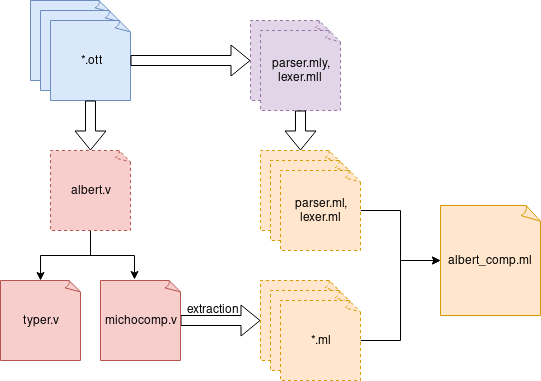
\includegraphics[height=5cm]{ressources/albert_comp.png}\\
  Almost all the code is extracted from Coq or generated from Ott.
\end{frame}

\begin{frame}{Compiler pipeline}
  \begin{enumerate}
  \item Inlining of type definitions
  \item Sorting of record and variant fields
  \item Type-checking (adds some type annotations)
  \item Compilation to MiChoCoq + function inlining
  \end{enumerate}
  Every step returns in an error monad (although compilation should not fail)
\end{frame}

\begin{frame}[fragile]{Stack manipulations}
  Carry a representation of the stack (list of the variable names) during the compilation.

  Use !DIG! and !DUG!

  Examples:\\
  $[[$?y = x?$|]$ = !DIG x ; DUG y!\\
  $[|$?x + y?$|]$ = !DIG y ; DIG x ; ADD!\\
\end{frame} 

\begin{frame}[fragile]{Why DUG}
  \begin{lstlisting}[language=albert]
    match b with
    True u -> x = 14; y = ``Hello''
    | False u -> y = ``World''; x = 42
    end
  \end{lstlisting}
  is of type ?{ b : bool } -> { u : unit ; x : nat ; y : string }?

  and compiles to !DIG b; IF { ... } { ... }!

  Without !DUG!ing, output stacks would be\\
  !nat::string::unit::S! and !string::nat::unit::S!

  Other solution: reorganize Albert's instructions (probably more efficient).
\end{frame}

%% \begin{frame}[fragile]{More complex compilations}
%%   \begin{tabular}{p{4.8cm}|p{8cm}}
%%     Albert code & Michelson code\\
%%     \hline
%%     $\{$x_1 = var_1 ; ... ; x_n = var_n$\} = $ & !UNPAIR; DUG var_1 ; ... ; DUG var_n!\\
%% \hline
%%   ?match var with?\newline$c_1$ $x_1$ ?->? $i_1$?|? \ldots\newline?|? $c_k$ $x_k$ ?->? $i_k$ ?end? &
%%   !DIG var ; ! \newline
%%   !IF_LEFT { DUG x_1 ;! $[|i_1|]$ !} { IF_LEFT !\ldots! }!\\
%% \hline
%%   \end{tabular}
%% \end{frame}

\section{Conclusion}

\begin{frame}{Accomplished work}
  \begin{itemize}
  \item Additions to MiChoCoq (DIG and DUG instructions, Micheline pretty-printer)
  \item Some improvements on Ott (in particular on the lexer and parser generators)
  \item Formal semantics of Albert in Ott
  \item Type-checker + compiler for almost all Albert (missing sets and some domain specific operations)
  \end{itemize}
\end{frame}

\begin{frame}{Future works}
  \begin{itemize}
  \item Proving type-checker and compiler properties
  \item Better error messages (locations)
  \item Optimization of stack manipulations
  \item And of course, writing compilers to Albert
  \end{itemize}
\end{frame}

\end{document}
